\section{Desenvolvimento Seguro}
Este capítulo apresenta uma visão inicial sobre algumas práticas comuns que podem melhorar a segurança das informações contidas no sistema. É um tema que está em constante mudança: a cada dia surgem novos tipos de ataques, novas vulnerabilidades são descobertas, técnicas aprimoradas. Enfim, essas práticas devem ser levadas em consideração apenas como ponto de partida.

\subsection{Principais Problemas}
Com o advento da computação, nos anos 1980, questões de segurança eram dificilmente levadas em consideração, porém a partir do momento em que os dispositivos móveis com algum tipo de informação sensível passaram a ter acesso à internet, a segurança dos dados se torna uma questão importante. \cite{DWIVEDI}. E assumir que o dispositivo poderá ser acessado por pessoas não confiáveis é o passo inicial para se preocupar com esse tipo de questão. 

A maior parte desse trabalho é feita pelos próprios fabricantes que disponibilizam o Sistema Operacional, mas o desenvolvedor também deve estar atento a alguns aspectos. 

A seguir, serão apresentados alguns cenários que possuem riscos potenciais no que diz respeito à segurança da informação.

\subsubsection{Segurança Física}
O termo “dispositivos móveis” remete à mobilidade que os mesmos trazem consigo, o que, por outro ponto de vista, pode significar um risco no que diz respeito à roubos ou perdas dos equipamentos. O que pode acontecer, no melhor caso, é a perda do valor pago no dispositivo em questão; porém, o pior cenário é o acesso a informações sensíveis contidas no aparelho, que em muitos casos pode valer até mais do que o próprio dispositivo e as consequências disso são até mesmo difíceis de mensurar. \cite{DWIVEDI} E, como já foi mencionado anteriormente, os dispositivos Apple possuem um mecanismo de segurança para esses casos.

\subsubsection{ Armazenamento Seguro de Dados}
A possibilidade de pessoas mal intencionadas terem acesso à algum dispositivo móvel é real. Seja algum conhecido ou até mesmo desconhecido, e basta que se tenha acesso por um pequeno momento apenas para que os dados contidos no dispositivo estajam em risco. Porém, isso deixa de ser um problema a partir do momento em que estes dados estão protegidos por algum mecanismo, seja por uma senha ou criptografados. Tratar essa possibilidade garantindo que apenas as aplicações e/ou donos da informação tenham acesso quando necessário é um ponto importante. \cite{DWIVEDI}

\subsubsection{Sistemas Operacionais Seguros}
Proteger um Sistema Operacional é uma tarefa difícil mas necessária. Porém quanto mais seguro for, melhor será a experiência do usuário. Pois a segurança muitas vezes está relacionada com a perda de informações, inatividade do sistema, etc. E quanto mais simples for para o usuário resolver esse tipo de problema, melhor. \cite{DWIVEDI}

\subsubsection{ Isolamento de Aplicações}
Existe uma infinidade de tipos de aplicativos que podem ser instalados, e na maioria dos casos, eles diferem bastante de um dispositivo para o outro. Cada tipo de aplicativo, para funcionar conforme esperado, precisa de um nível de acesso diferentes às informações e recursos do dispositivo. A capacidade de isolar essas aplicações e os dados de que cada uma necessita é um passo importante para garantir que um aplicativo não autorizado tenha acesso aos dados de outros. \cite{DWIVEDI}

\subsubsection{Divulgação de Informações}
A segurança da informação está diretamente relacionada com a proteção de dados sensíveis, evitar que os mesmos sejam divulgados é essencial. 

Se, por qualquer motivo, alguma pessoa não confiável tiver acesso à informações, o risco das mesmas serem divulgadas é real. Esta é uma questão importante para tratar e mitigar. \cite{DWIVEDI} 

\subsubsection{Vírus, Worms, Trojans, Spyware e Malware}
Em qualquer dispositivo que possua algum tipo de conexão externa, essas ameaças podem representar um risco à segurança dos dados contidos no mesmo. A capacidade de se adaptar às mudanças levando em consideração os anos de conhecimentos anteriores sobre o tema em outras plataformas é crucial para a criação de aplicações e sistemas operacionais mais seguros. \cite{DWIVEDI} 

\subsubsection{Fraude Eletrônica (Phishing)}
É um grande problema em dispositivos móveis. Principalmente por que alguns usuários clicam em itens sem pensar, ou sem saber o que estão fazendo. Nos dispositivos móveis em especial, muitos navegadores de internet colapsam a URL do site que está sendo acessado. Com isso, os usuários podem facilmente serem vítimas de fraudes. \cite{DWIVEDI}  

O phishing funciona da seguinte forma: um site idêntico ao de um banco, por exemplo, é criado e ao tentar acessar o site original a partir do celular, ele aparece e os dados da conta e senha do banco são inseridos, ao tentar acessar a conta aparece uma mensagem de erro, mesmo que os dados estejam corretos. Neste ponto as informações são enviadas pra algum servidor de terceiros e o site falso redireciona o usuário para o site original. Que ao tentar acessar novamente, terá sucesso. Muitas pessoas só percebem que foram vítimas quando vão verificar a fatura do cartão de crédito ou saldo na conta, muito tempo depois de ter acontecido. 

\subsubsection{ Privacidade e Serviços de Localização}
Como citado anteriormente, a maioria dos dispositivos atuais possuem GPS integrado e, com isso, é possível saber onde o usuário está. Grande parte desses usuários desejam privacidade, mas sem perceber compartilham sua localização com aplicativos de Mapa ou Redes Sociais e desconsideram o cenário em que possam estar sendo observados. 

Quase todos esses aplicativos permitem que o usuário escolha com quem deseja compartilhar essa informação ou tratam esses dados de forma anônima, mas existe a possibilidade de pessoas ou aplicativos não confiáveis terem más intenções. Há, naturalmente, o caso em que se observam políticas de uso que abertamente declaram que irão usar esses dados, todavia o usuário, por omissão, não lê na íntegra o documento e fica exposto aos efeitos adversos e muitas vezes indesejados da política de uso do fornecedor. 

Então para que a utilização desta tecnologia não represente um risco, é importante ter bastante cuidado. \cite{DWIVEDI} 

\subsection{Boas Práticas}
A segurança no desenvolvimento de software deve levar em consideração diversos fatores, é necessário bem mais do que pessoas tecnicamente capacitadas na linguagem e máquinas super potentes para criar aplicações com certo nível de segurança. Tomar como base um método de desenvolvimento seguro é crucial para aumentar a confiabilidade do sistema; além disso, há alguns princípios de computação segura que devem ser também levados em consideração.
A seguir serão listadas algumas boas práticas que, se seguidas, ajudarão e muito nesse propósito.

\subsubsection{Seguir Práticas de Programação Segura}
Estudar a linguagem na qual o aplicativo será desenvolvido é importante. Saber quais são as nuances e práticas de segurança que a linguagem oferece também. Para isso, tempo e experiência na linguagem contam bastante. Apesar de que muitas vezes, os aplicativos precisam ser entregues em pouco tempo, não se pode ignorar testes e verificações de segurança, pois um produto potencialmente inseguro pode significar um problema no futuro. 

A maior parte das linguagens possuem documentação extensa e guias para uma programação segura. O aproveitamento dessas informações é importante para fazer um código o mais seguro possível. E ainda evitar que erros comuns sejam praticados. \cite{DWIVEDI} 
\subsubsection{Validar as Entradas de Informações}
A validação das entradas de informações vem desde o advento da programação web nos anos 2000. E, desde então, é uma recomendação padrão da maioria das linguagens. Nos dispositivos móveis, as entradas de dados variam bastante, deixando apenas de ser um text field para um picker, switch, table, etc. A importância de se validar as entradas não pode ser subestimada.\cite{DWIVEDI}

\subsubsection{ Utilize os Privilégios Mínimos Necessários}
Permissões de acesso a recursos do dispositivo, tais como GPS, Internet, Contatos, Fotos, etc., devem ser os mínimos possíveis. Não faz sentido algum uma aplicação cujo objetivo é apenas publicar fotos em alguma rede social, solicitar permissão de acesso aos contatos ou mensagens do dispositivo. Este modelo de menor privilégio possível envolve apenas pedir o que é estritamente necessário para o funcionamento da aplicação. E a sua adoção garante que um aplicativo não afete os outros instalados no dispositivo e que os recursos funcionem da forma como deveriam. \cite{DWIVEDI}

\subsubsection{Armazene Informações Corretamente}
É recomendado evitar o armazenamento de informações confidenciais, como nomes de usuário ou senhas, em textos simples no dispositivo ou em algum local de fácil acesso. Utilize os recursos de criptografia e banco de dados provenientes da plataforma, que permitem que os aplicativos armazenem tais informações com segurança e sem a necessidade de utilizar softwares de terceiros. \cite{DWIVEDI}

\subsubsection{Evite Ameaças Comuns}
Embora ameaças para aplicações móveis sejam reais, é importante saber distinguir qual tipo de ameaça realmente devem ser levadas em consideração para o contexto da aplicação. Qualquer livro de segurança apresenta várias ameaças e entender como cada uma delas funciona e quais delas podem representar um risco é necessário. A melhor maneira de iniciar esse processo é conhecer e listar essas potenciais ameaças, desenhar processos de mitigação e observar as demais como riscos aceitos. Esse processo é comumente conhecido como “Modelo de Ameaça para o Aplicativo”. Que não deve ser exaustivo ou super completo, basta servir como um guia para os desenvolvedores entenderem como tratar cada tipo de ameaça. \cite{DWIVEDI}

\begin{figure}[h]
\centering
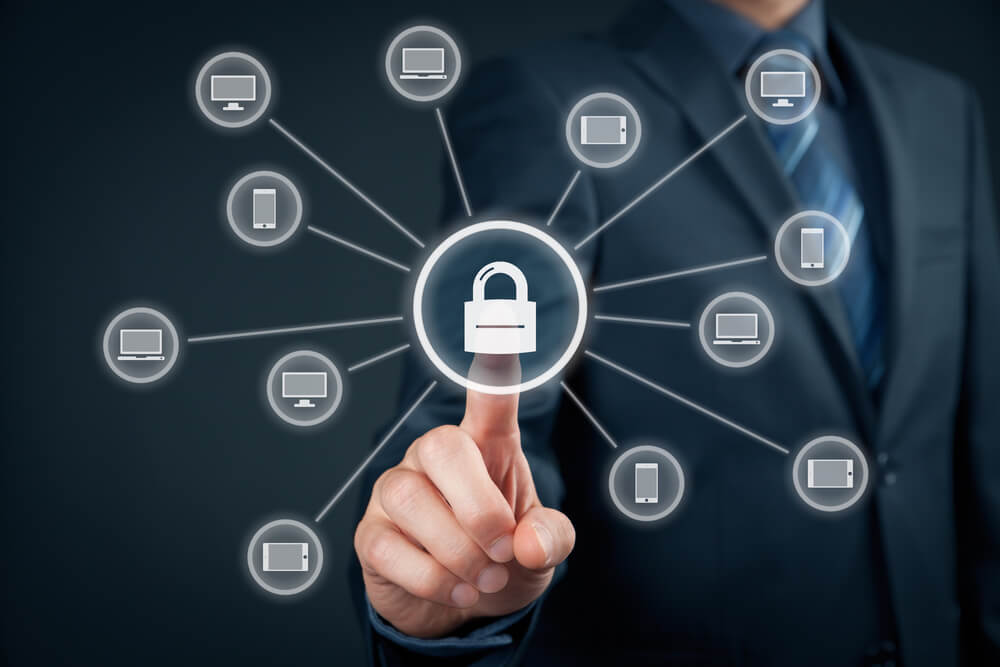
\includegraphics[width=.5\textwidth]{secoes/figuras/img1.jpg}
\caption{Tecnologia e Segurança.}
\label{figura1}
\end{figure}